%%%% Paramétrage du TD %%%%
\def\xxactivite{\ifcolle Colle \else Application 04 \fi \ifprof -- Corrigé \else \fi }
\def\xxauteur{\textsl{Xavier Pessoles}}


\def\xxnumchapitre{Révisions 5 \vspace{.2cm}}
\def\xxchapitre{\hspace{.12cm} Modélisation des systèmes linéaires -- Domaine fréquentiel}

\def\xxcompetences{%
\vspace{-.5cm}
\footnotesize{
\textsl{%
\textbf{Savoirs et compétences :}\\
\vspace{-.2cm}
\begin{itemize}[label=\ding{112},font=\color{ocre}] 
\item ...
\end{itemize}}}}

\def\xxfigures{
%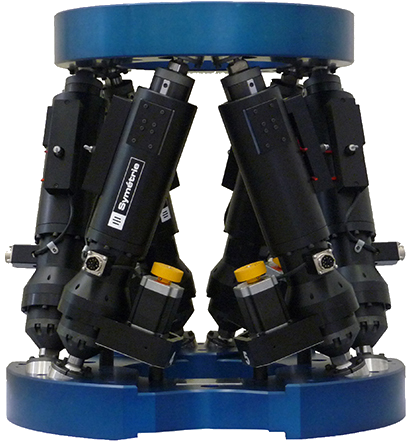
\includegraphics[width=.3\textwidth]{fig_01}
}%figues de la page de garde

\def\xxtitreexo{Applications}
\def\xxsourceexo{D'après Sébastien Grange}

\iflivret
\pagestyle{empty}


%%%%%%%% PAGE DE GARDE COURS
\ifcours
% ==== BANDEAU DES TITRES ==== 
\begin{tikzpicture}[remember picture,overlay]
\node at (current page.north west)
{\begin{tikzpicture}[remember picture,overlay]
\node[anchor=north west,inner sep=0pt] at (0,0) {\includegraphics[width=\paperwidth]{\thechapterimage}};
\draw[anchor=west] (-2cm,-8cm) node [line width=2pt,rounded corners=15pt,draw=ocre,fill=white,fill opacity=0.6,inner sep=40pt]{\strut\makebox[22cm]{}};
\draw[anchor=west] (1cm,-8cm) node {\huge\sffamily\bfseries\color{black} %
\begin{minipage}{1cm}
\rotatebox{90}{\LARGE\sffamily\textsc{\color{ocre}\textbf{\xxnumpartie}}}
\end{minipage} \hfill
\begin{minipage}[c]{14cm}
\begin{titrepartie}
\begin{flushright}
\renewcommand{\baselinestretch}{1.1} 
\Large\sffamily\textsc{\textbf{\xxpartie}}
\renewcommand{\baselinestretch}{1} 
\end{flushright}
\end{titrepartie}
\end{minipage} \hfill
\begin{minipage}[c]{3.5cm}
{\large\sffamily\textsc{\textbf{\color{ocre} \discipline}}}
\end{minipage} 
 };
\end{tikzpicture}};
\end{tikzpicture}
% ==== FIN BANDEAU DES TITRES ==== 


% ==== ONGLET 
\begin{tikzpicture}[overlay]
\node[shape=rectangle, 
      rounded corners = .25 cm,
	  draw= ocre,
	  line width=2pt, 
	  fill = ocre!10,
	  minimum width  = 2.5cm,
	  minimum height = 3cm,] at (18.3cm,0) {};
\node at (17.7cm,0) {\rotatebox{90}{\textbf{\Large\color{ocre}{\classe}}}};
%{};
\end{tikzpicture}
% ==== FIN ONGLET 


\vspace{3.5cm}

\begin{tikzpicture}[remember picture,overlay]
\draw[anchor=west] (-2cm,-6cm) node {\huge\sffamily\bfseries\color{black} %
\begin{minipage}{2cm}
\begin{center}
\LARGE\sffamily\textsc{\color{ocre}\textbf{\xxactivite}}
\end{center}
\end{minipage} \hfill
\begin{minipage}[c]{15cm}
\begin{titrechapitre}
\renewcommand{\baselinestretch}{1.1} 
\Large\sffamily\textsc{\textbf{\xxnumchapitre}}

\Large\sffamily\textsc{\textbf{\xxchapitre}}
\vspace{.5cm}

\renewcommand{\baselinestretch}{1} 
\normalsize\normalfont
\xxcompetences
\end{titrechapitre}
\end{minipage}  };
\end{tikzpicture}
\vfill

\begin{flushright}
\begin{minipage}[c]{.3\linewidth}
\begin{center}
\xxfigures
\end{center}
\end{minipage}\hfill
\begin{minipage}[c]{.6\linewidth}
\startcontents
%\printcontents{}{1}{}
\printcontents{}{1}{}
\end{minipage}
\end{flushright}

\begin{tikzpicture}[remember picture,overlay]
\draw[anchor=west] (4.5cm,-.7cm) node {
\begin{minipage}[c]{.2\linewidth}
\begin{flushright}

\includegraphics[width=2cm]{logoCC}
\end{flushright}
\end{minipage}
\begin{minipage}[c]{.2\linewidth}
\textsl{\xxauteur} \\
\textsl{\classe}
\end{minipage}
 };
\end{tikzpicture}

\newpage
\pagestyle{fancy}

%\newpage
%\pagestyle{fancy}

\else
\fi
%% FIN PAGE DE GARDE DES COURS

%%%%%%%% PAGE DE GARDE TD
\iftd

% BANDEAU EXO
\iflivret % SI LIVRET
\begin{tikzpicture}[remember picture,overlay]
\draw[anchor=west] (-2cm,-3.3cm) node {\huge\sffamily\bfseries\color{black} %
\begin{minipage}{5cm}
\begin{center}
\LARGE\sffamily\color{ocre}\textbf{\textsc{\xxactivite}}

\begin{center}
\xxfigures
\end{center}

\end{center}
\end{minipage} \hfill
\begin{minipage}[c]{12cm}
\begin{titrechapitre}
\renewcommand{\baselinestretch}{1.1} 
\large\sffamily\textbf{\textsc{\xxtitreexo}}

\small\sffamily{\textbf{\textit{\color{black!70}\xxsourceexo}}}
\vspace{.5cm}

\renewcommand{\baselinestretch}{1} 
\normalsize\normalfont
\xxcompetences
\end{titrechapitre}
\end{minipage}};
\end{tikzpicture}
\else % ELSE NOT LIVRET
\begin{tikzpicture}[remember picture,overlay]
\draw[anchor=west] (-2cm,-4.5cm) node {\huge\sffamily\bfseries\color{black} %
\begin{minipage}{5cm}
\begin{center}
\LARGE\sffamily\color{ocre}\textbf{\textsc{\xxactivite}}

\begin{center}
\xxfigures
\end{center}

\end{center}
\end{minipage} \hfill
\begin{minipage}[c]{12cm}
\begin{titrechapitre}
\renewcommand{\baselinestretch}{1.1} 
\large\sffamily\textbf{\textsc{\xxtitreexo}}

\small\sffamily{\textbf{\textit{\color{black!70}\xxsourceexo}}}
\vspace{.5cm}

\renewcommand{\baselinestretch}{1} 
\normalsize\normalfont
\xxcompetences
\end{titrechapitre}
\end{minipage}};
\end{tikzpicture}

\fi

\else   % FIN IF TD
\fi


%%%%%%%% PAGE DE GARDE FICHE
\iffiche
\begin{tikzpicture}[remember picture,overlay]
\node at (current page.north west)
{\begin{tikzpicture}[remember picture,overlay]
\draw[anchor=west] (-2cm,-2.25cm) node [line width=2pt,rounded corners=15pt,draw=ocre,fill=white,fill opacity=0.6,inner sep=40pt]{\strut\makebox[22cm]{}};
\draw[anchor=west] (1cm,-2.25cm) node {\huge\sffamily\bfseries\color{black} %
\begin{minipage}{1cm}
\rotatebox{90}{\LARGE\sffamily\textsc{\color{ocre}\textbf{\xxnumpartie}}}
\end{minipage} \hfill
\begin{minipage}[c]{14cm}
\begin{titrepartie}
\begin{flushright}
\renewcommand{\baselinestretch}{1.1} 
\large\sffamily\textsc{\textbf{\xxpartie} \\} 

\vspace{.2cm}

\normalsize\sffamily\textsc{\textbf{\xxnumchapitre -- \xxchapitre}}
\renewcommand{\baselinestretch}{1} 
\end{flushright}
\end{titrepartie}
\end{minipage} \hfill
\begin{minipage}[c]{3.5cm}
{\large\sffamily\textsc{\textbf{\color{ocre} \discipline}}}
\end{minipage} 
 };
\end{tikzpicture}};
\end{tikzpicture}

\iflivret % SI LIVRET
\begin{tikzpicture}[overlay]
\node[shape=rectangle, 
      rounded corners = .25 cm,
	  draw= ocre,
	  line width=2pt, 
	  fill = ocre!10,
	  minimum width  = 2.5cm,
	  minimum height = 2.5cm,] at (18.5cm,.5cm) {};
\node at (17.9cm,.5cm) {\rotatebox{90}{\textsf{\textbf{\large\color{ocre}{\classe}}}}};
%{};
\end{tikzpicture}
\else  % SI PAS LIVRET
\iftd %% SI TD et PAS LIVRET
\begin{tikzpicture}[overlay]
\node[shape=rectangle, 
      rounded corners = .25 cm,
	  draw= ocre,
	  line width=2pt, 
	  fill = ocre!10,
	  minimum width  = 2.5cm,
	  minimum height = 2.5cm,] at (18.6cm,0.9cm) {};
\node at (18cm,0.9cm) {\rotatebox{90}{\textsf{\textbf{\large\color{ocre}{\classe}}}}};
%{};
\end{tikzpicture}

\else % FIN DU SI TD PAS LIVRET 
\begin{tikzpicture}[overlay]
\node[shape=rectangle, 
      rounded corners = .25 cm,
	  draw= ocre,
	  line width=2pt, 
	  fill = ocre!10,
	  minimum width  = 2.5cm,
%	  minimum height = 2.5cm,] at (18.5cm,1.1cm) {};
	  minimum height = 2.5cm,] at (18.6cm,0.5cm) {};
\node at (18cm,0.5cm) {\rotatebox{90}{\textsf{\textbf{\large\color{ocre}{\classe}}}}};
%{};
\end{tikzpicture}
\fi
\fi
\else
\fi



\else
\pagestyle{empty}


%%%%%%%% PAGE DE GARDE COURS
\ifcours
% ==== BANDEAU DES TITRES ==== 
\begin{tikzpicture}[remember picture,overlay]
\node at (current page.north west)
{\begin{tikzpicture}[remember picture,overlay]
\node[anchor=north west,inner sep=0pt] at (0,0) {\includegraphics[width=\paperwidth]{\thechapterimage}};
\draw[anchor=west] (-2cm,-8cm) node [line width=2pt,rounded corners=15pt,draw=ocre,fill=white,fill opacity=0.6,inner sep=40pt]{\strut\makebox[22cm]{}};
\draw[anchor=west] (1cm,-8cm) node {\huge\sffamily\bfseries\color{black} %
\begin{minipage}{1cm}
\rotatebox{90}{\LARGE\sffamily\textsc{\color{ocre}\textbf{\xxnumpartie}}}
\end{minipage} \hfill
\begin{minipage}[c]{14cm}
\begin{titrepartie}
\begin{flushright}
\renewcommand{\baselinestretch}{1.1} 
\Large\sffamily\textsc{\textbf{\xxpartie}}
\renewcommand{\baselinestretch}{1} 
\end{flushright}
\end{titrepartie}
\end{minipage} \hfill
\begin{minipage}[c]{3.5cm}
{\large\sffamily\textsc{\textbf{\color{ocre} \discipline}}}
\end{minipage} 
 };
\end{tikzpicture}};
\end{tikzpicture}
% ==== FIN BANDEAU DES TITRES ==== 


% ==== ONGLET 
\begin{tikzpicture}[overlay]
\node[shape=rectangle, 
      rounded corners = .25 cm,
	  draw= ocre,
	  line width=2pt, 
	  fill = ocre!10,
	  minimum width  = 2.5cm,
	  minimum height = 3cm,] at (18.3cm,0) {};
\node at (17.7cm,0) {\rotatebox{90}{\textbf{\Large\color{ocre}{\classe}}}};
%{};
\end{tikzpicture}
% ==== FIN ONGLET 


\vspace{3.5cm}

\begin{tikzpicture}[remember picture,overlay]
\draw[anchor=west] (-2cm,-6cm) node {\huge\sffamily\bfseries\color{black} %
\begin{minipage}{2cm}
\begin{center}
\LARGE\sffamily\textsc{\color{ocre}\textbf{\xxactivite}}
\end{center}
\end{minipage} \hfill
\begin{minipage}[c]{15cm}
\begin{titrechapitre}
\renewcommand{\baselinestretch}{1.1} 
\Large\sffamily\textsc{\textbf{\xxnumchapitre}}

\Large\sffamily\textsc{\textbf{\xxchapitre}}
\vspace{.5cm}

\renewcommand{\baselinestretch}{1} 
\normalsize\normalfont
\xxcompetences
\end{titrechapitre}
\end{minipage}  };
\end{tikzpicture}
\vfill

\begin{flushright}
\begin{minipage}[c]{.3\linewidth}
\begin{center}
\xxfigures
\end{center}
\end{minipage}\hfill
\begin{minipage}[c]{.6\linewidth}
\startcontents
%\printcontents{}{1}{}
\printcontents{}{1}{}
\end{minipage}
\end{flushright}

\begin{tikzpicture}[remember picture,overlay]
\draw[anchor=west] (4.5cm,-.7cm) node {
\begin{minipage}[c]{.2\linewidth}
\begin{flushright}

\includegraphics[width=2cm]{logoCC}
\end{flushright}
\end{minipage}
\begin{minipage}[c]{.2\linewidth}
\textsl{\xxauteur} \\
\textsl{\classe}
\end{minipage}
 };
\end{tikzpicture}

\newpage
\pagestyle{fancy}

%\newpage
%\pagestyle{fancy}

\else
\fi
%% FIN PAGE DE GARDE DES COURS

%%%%%%%% PAGE DE GARDE TD
\iftd

% BANDEAU EXO
\iflivret % SI LIVRET
\begin{tikzpicture}[remember picture,overlay]
\draw[anchor=west] (-2cm,-3.3cm) node {\huge\sffamily\bfseries\color{black} %
\begin{minipage}{5cm}
\begin{center}
\LARGE\sffamily\color{ocre}\textbf{\textsc{\xxactivite}}

\begin{center}
\xxfigures
\end{center}

\end{center}
\end{minipage} \hfill
\begin{minipage}[c]{12cm}
\begin{titrechapitre}
\renewcommand{\baselinestretch}{1.1} 
\large\sffamily\textbf{\textsc{\xxtitreexo}}

\small\sffamily{\textbf{\textit{\color{black!70}\xxsourceexo}}}
\vspace{.5cm}

\renewcommand{\baselinestretch}{1} 
\normalsize\normalfont
\xxcompetences
\end{titrechapitre}
\end{minipage}};
\end{tikzpicture}
\else % ELSE NOT LIVRET
\begin{tikzpicture}[remember picture,overlay]
\draw[anchor=west] (-2cm,-4.5cm) node {\huge\sffamily\bfseries\color{black} %
\begin{minipage}{5cm}
\begin{center}
\LARGE\sffamily\color{ocre}\textbf{\textsc{\xxactivite}}

\begin{center}
\xxfigures
\end{center}

\end{center}
\end{minipage} \hfill
\begin{minipage}[c]{12cm}
\begin{titrechapitre}
\renewcommand{\baselinestretch}{1.1} 
\large\sffamily\textbf{\textsc{\xxtitreexo}}

\small\sffamily{\textbf{\textit{\color{black!70}\xxsourceexo}}}
\vspace{.5cm}

\renewcommand{\baselinestretch}{1} 
\normalsize\normalfont
\xxcompetences
\end{titrechapitre}
\end{minipage}};
\end{tikzpicture}

\fi

\else   % FIN IF TD
\fi


%%%%%%%% PAGE DE GARDE FICHE
\iffiche
\begin{tikzpicture}[remember picture,overlay]
\node at (current page.north west)
{\begin{tikzpicture}[remember picture,overlay]
\draw[anchor=west] (-2cm,-2.25cm) node [line width=2pt,rounded corners=15pt,draw=ocre,fill=white,fill opacity=0.6,inner sep=40pt]{\strut\makebox[22cm]{}};
\draw[anchor=west] (1cm,-2.25cm) node {\huge\sffamily\bfseries\color{black} %
\begin{minipage}{1cm}
\rotatebox{90}{\LARGE\sffamily\textsc{\color{ocre}\textbf{\xxnumpartie}}}
\end{minipage} \hfill
\begin{minipage}[c]{14cm}
\begin{titrepartie}
\begin{flushright}
\renewcommand{\baselinestretch}{1.1} 
\large\sffamily\textsc{\textbf{\xxpartie} \\} 

\vspace{.2cm}

\normalsize\sffamily\textsc{\textbf{\xxnumchapitre -- \xxchapitre}}
\renewcommand{\baselinestretch}{1} 
\end{flushright}
\end{titrepartie}
\end{minipage} \hfill
\begin{minipage}[c]{3.5cm}
{\large\sffamily\textsc{\textbf{\color{ocre} \discipline}}}
\end{minipage} 
 };
\end{tikzpicture}};
\end{tikzpicture}

\iflivret % SI LIVRET
\begin{tikzpicture}[overlay]
\node[shape=rectangle, 
      rounded corners = .25 cm,
	  draw= ocre,
	  line width=2pt, 
	  fill = ocre!10,
	  minimum width  = 2.5cm,
	  minimum height = 2.5cm,] at (18.5cm,.5cm) {};
\node at (17.9cm,.5cm) {\rotatebox{90}{\textsf{\textbf{\large\color{ocre}{\classe}}}}};
%{};
\end{tikzpicture}
\else  % SI PAS LIVRET
\iftd %% SI TD et PAS LIVRET
\begin{tikzpicture}[overlay]
\node[shape=rectangle, 
      rounded corners = .25 cm,
	  draw= ocre,
	  line width=2pt, 
	  fill = ocre!10,
	  minimum width  = 2.5cm,
	  minimum height = 2.5cm,] at (18.6cm,0.9cm) {};
\node at (18cm,0.9cm) {\rotatebox{90}{\textsf{\textbf{\large\color{ocre}{\classe}}}}};
%{};
\end{tikzpicture}

\else % FIN DU SI TD PAS LIVRET 
\begin{tikzpicture}[overlay]
\node[shape=rectangle, 
      rounded corners = .25 cm,
	  draw= ocre,
	  line width=2pt, 
	  fill = ocre!10,
	  minimum width  = 2.5cm,
%	  minimum height = 2.5cm,] at (18.5cm,1.1cm) {};
	  minimum height = 2.5cm,] at (18.6cm,0.5cm) {};
\node at (18cm,0.5cm) {\rotatebox{90}{\textsf{\textbf{\large\color{ocre}{\classe}}}}};
%{};
\end{tikzpicture}
\fi
\fi
\else
\fi



\fi
\setlength{\columnseprule}{.1pt}

\pagestyle{fancy}
\thispagestyle{plain}


\vspace{3.5cm}

\def\columnseprulecolor{\color{ocre}}
\setlength{\columnseprule}{0.4pt} 

%%%%%%%%%%%%%%%%%%%%%%%

\ifprof
\else
%\begin{multicols}{2}
\fi


\section*{Diagramme de Bode}
\subparagraph{}
\textit{Tracer les diagrammes de Bode réels et asymptotiques de la fonction de transfert suivante : }
$$
H(p)=\dfrac{0,6}{(p+0.025)(p^2+0,2p+1)}
$$

\ifprof
\begin{corrige}
$H(p)=\dfrac{0,6}{(p+0,025)(p^2+0,2p+1)}=\dfrac{24}{(1+40p)\left(1+\dfrac{2\cdot 0,1}{1} p+\dfrac{p^2}{1^2}\right)}$
\end{corrige}
\begin{center}
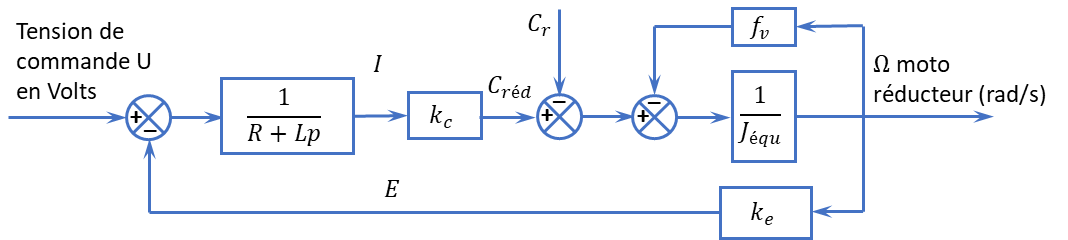
\includegraphics[width=.8\linewidth]{cor_01}
\end{center}

\else
\begin{center}
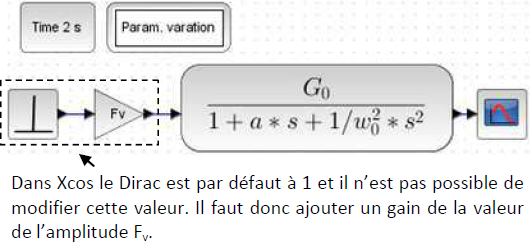
\includegraphics[width=.8\linewidth]{img_04}
\end{center}
\fi

%\newpage
\subparagraph{}
\textit{Tracer les diagrammes de Bode réel et asymptotique de la fonction de transfert suivante : }
$$
H(p)=\dfrac{5(p+60)}{p(p^2+5p+4)}
$$


\ifprof
\begin{corrige} ~\\

$H(p)=\dfrac{5(p+60)}{p(p^2+5p+4)} =\dfrac{75(1+0,0167p)}{p(1+(2\cdot 1,25)/2 p+p^2/2^2 )} =\dfrac{75(1+0,0167p)}{p(1+p)(1+0,25p)}
$
\end{corrige}
\begin{center}
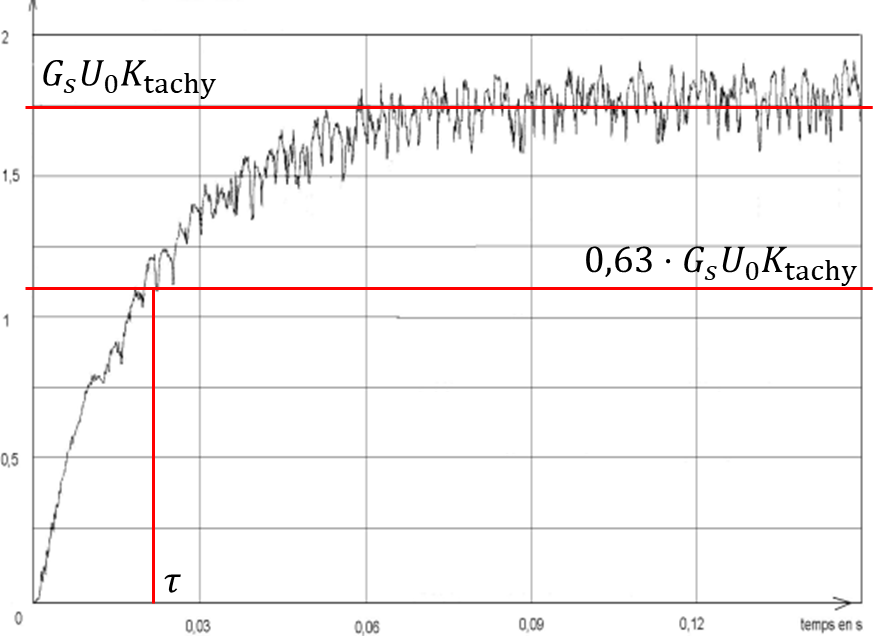
\includegraphics[width=.8\linewidth]{cor_02}
\end{center}
\else
\begin{center}
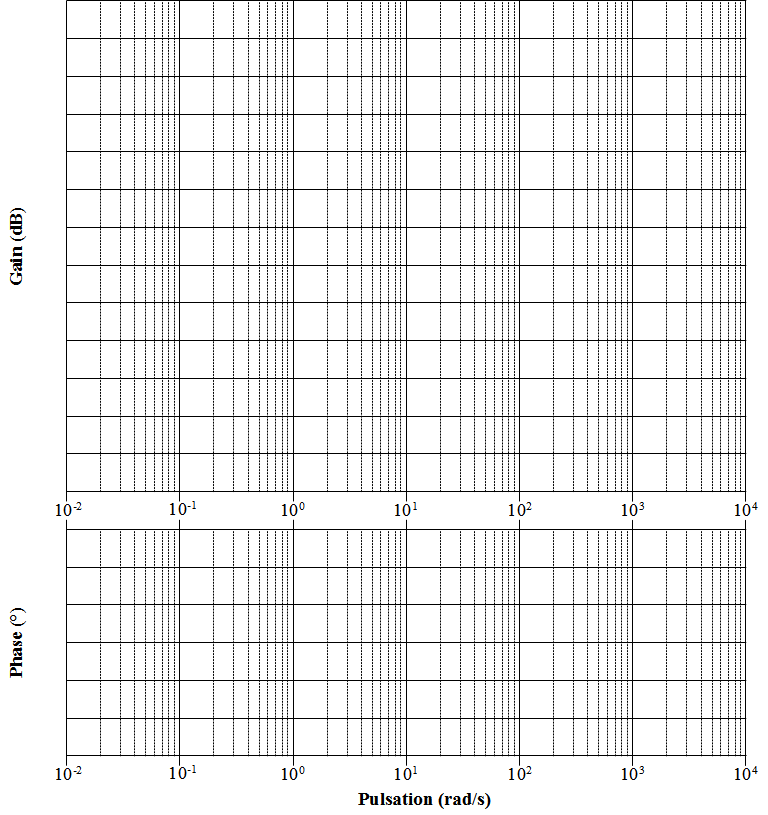
\includegraphics[width=.8\linewidth]{img_05}
\end{center}\fi



%\newpage

\subparagraph{}
\textit{Identifier la fonction de transfert représentée par le diagramme de Bode suivant. Vous justifierez notamment sa forme :$H(p)=\dfrac{K}{p(1+T_1 p)(1+T_2 p)}$. Donner les deux pôles dominants, en déduire une expression simplifiée de $H(p)$. }

\ifprof
\begin{corrige}
D’après le diagramme de Bode, on voit que la fonction de transfert possède un intégrateur puisque la phase débute à 90 degrés. De plus la phase diminue dans un premier temps de 90 degrés puis encore de 90degrés ce qui justifie les 2 1\ier ordres.

Pour identifier les constantes de temps, on va utiliser le fait que la phase d’un premier ordre passe par -45 degrés pour sa pulsation de coupure qui vaut $\dfrac{1}{\tau}$.
Ici, il y a un intégrateur. On trouve donc les pulsations de coupure lorsque la phase vaut -135 degrés puis -225 degrés. On a :
$1/T_1 \simeq 100$      et      $1/T_2 \simeq 2000$     donc    $T_1=\SI{0.01}{s}$ et
$T_2=\SI{0.0005}{s}$.

Pour identifier le gain, on se place pour des pulsations faibles, ici $\omega =0,1 rad/s$. Pour ces pulsations, on sait que les gains des 1\ier{} ordre valent environ $20\log K$ et celui de l’intégrateur $20\log(1⁄\omega)$. On a donc pour $\omega=0,1 rad/s$ :
$20 \log(K⁄0,1) \simeq -20 $  $K\simeq 1$

On a donc : $H(p)=\dfrac{1}{p(1+0.01p)(1+0.0005p)}$.

Le pôle dominant est le pôle qui met le plus de temps à converger, c’est-à-dire celui qui a la constante de temps la plus grande, on a donc :
$H(p)\simeq \dfrac{1}{p(1+0.01p)}$.
\end{corrige}
\else
\begin{center}
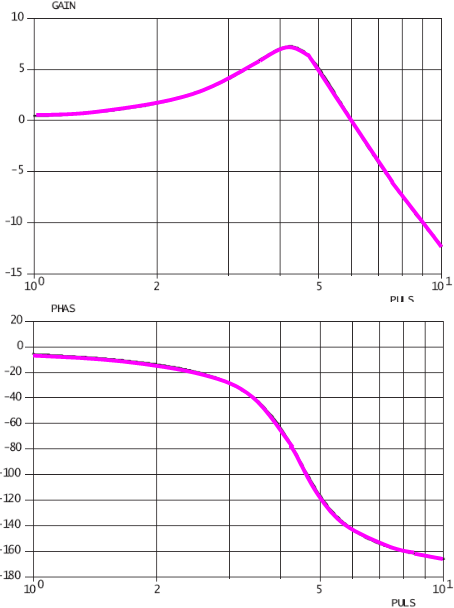
\includegraphics[width=.8\linewidth]{img_01}
\end{center}
\fi

\subparagraph{}
\textit{On suppose que l'entrée du système est sinusoïdale : $e(t)=3\sin 300 t$. Donner
 l'expression de la réponse en régime permanent à partir ce même diagramme de Bode.}
%\end{multicols}

\ifprof
\begin{corrige}
On sait que la sortie sera également sinusoïdale, de même pulsation que l’entrée mais déphasée et d’amplitude différente : $s(t)=S_0 \sin \left(300t +\varphi\right)$.

Le diagramme de Bode nous donne le rapport de l’amplitude entre la sortie et l’entrée (courbe de gain) et le déphasage de la sortie par rapport à l’entrée (courbe de phase).

$G_{dB} (\omega=300 rad/s)=20\log(S_0/E_0 )=20\log(S_0/3)$.

On peut lire que :
$G_{dB} (\omega =300 rad/s)\simeq -\SI{60}{dB}$ et donc $S_0\simeq 3 \cdot 10^{-3}$.
D’après la courbe de phase, on peut lire :
$\varphi (\omega=300 rad/s)=-\SI{175}{degr\'es}$
On a donc : $s(t)=3\cdot 10^{-3} \sin\left( 300t -3,05\right)$.
L’angle est à mettre en radians.

\end{corrige}
\else
\fi

%\newpage 

\subparagraph{}
\textit{Identifier la fonction de transfert représentée par le diagramme de Bode suivant. La calculatrice est autorisée.
On rappelle que pour une fonction de transfert du 2ème ordre, on a : $\text{Max}\left(G_{\text{dB}} \right)=20\log\dfrac{K}{2\xi\sqrt{1-\xi^2}}$.}

\ifprof
\begin{corrige}
D’après le diagramme de Bode, on voit que la fonction de transfert possède un intégrateur puisque la phase débute à 90 degrés. Ensuite la phase augmente dans un premier temps de 90 degrés, ce qui signifie la présente d’un « 1er ordre » en numérateur. Puis la phase diminue de 180 degrés  et le gain résonne ce qui justifie la présence d’un 2ème ordre avec un coefficient d’amortissement plus petit que $1⁄\sqrt{2}$.

$H(p)=\dfrac{K(1+Tp)}{p(1+2\xi/\omega_0  p+p^2/(\omega^2 ))}$

Pour identifier la constante de temps, on va utiliser le fait que la phase d’un « premier ordre » au numérateur passe par 45 degrés pour sa pulsation de coupure qui vaut $1⁄\tau$.
Ici, il y a un intégrateur. On trouve donc la pulsation de coupure lorsque la phase vaut -45 degrés. On a :
$1/T\simeq 1$ et $T=\SI{1}{s}$.

Pour identifier la pulsation de coupure, on va utiliser le fait que la phase d’un 2ème ordre passe par -90 degrés pour sa pulsation de coupure qui vaut $\omega_0$.
Ici, il y a un intégrateur et un « 1er ordre » au numérateur. On trouve donc la pulsation de coupure lorsque la phase vaut -90 degrés. On a :
$\omega_0\simeq \SI{80}{rad/s}$.

Pour identifier le coefficient d’amortissement, on va utiliser la résonnance. On a :
$20\log(1/(2\xi\sqrt{1-\xi^2 }))\simeq 13$ et $\xi\simeq 0,11$.

Pour identifier le gain, on se place pour des pulsations faibles, ici $\omega=0,1 rad/s$. Pour ces pulsations, on sait que les gains des 1er ordre et du 2ème ordre valent environ $20\log K$ et celui de l’intégrateur $20\log(1⁄\omega)$. On a donc pour $\omega=\SI{0,1}{rad/s}$ :
$20\log(K⁄0.1)\simeq 33$ et $K\simeq4.5$

\end{corrige}
\else

\begin{center}
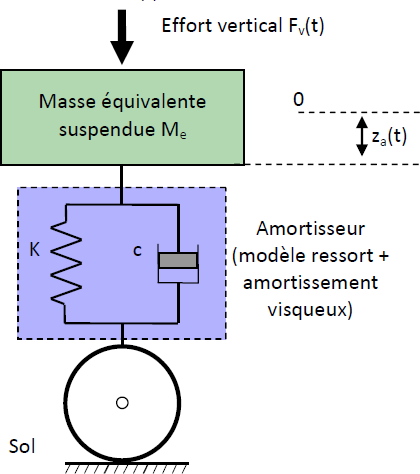
\includegraphics[width=.8\linewidth]{img_02}
\end{center}
\fi

\subparagraph{}
\textit{Déterminer les marges de stabilité pour ces quatre fonctions de transfert.}

%Pour la question 1 :
%H(p)=0.6/(p+0.025)(p^2+0.2p+1) 
%Le système est instable, il n’y a pas de marges de stabilité.
%
%Pour la question 2 :
%H(p)=5(p+60)/p(p^2+5p+4) 
%Le système est instable, il n’y a pas de marges de stabilité.
%
%Pour la question 3 :
%H(p)=1/p(1+0.01p)(1+0.0005p) 
%On a :
%MG≈70dB     et     Mφ≈90°
%
%Pour la question 4 :
%H(p)=4.5(1+p)/p(1+(2∙0.11)/80 p+p^2/〖80〗^2 ) 
%Le système est instable, il n’y a pas de marges de stabilité.
%

%\newpage

\section*{Réponse fréquentielle}
\setcounter{exo}{0}
Un capteur d'accélération de sensibilité S est utilisé dans la chaîne de retour d'un système asservi dont l'objectif est de contrôler l'accélération d'un plateau sur lequel est fixé ce capteur. Le moteur permettant la motorisation du plateau est connu par l'intermédiaire de sa fonction de transfert. 


\begin{center}
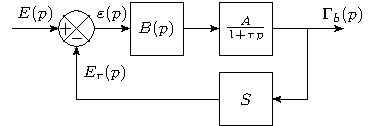
\includegraphics{Schema_1_entree_2F_R}
\end{center}

On a  $A = \SI{100}{g.m.s^{-2}.V^{-1}}$, $\tau=\SI{0,2}{s}$ et $S = 10\cdot 10^{-3}/g V/(m/s^2)$ où $g$ est l'accélération de pesanteur. $E(p)$ est la transformée de Laplace de $e(t)$ la tension de consigne de cet asservissement et $\Gamma_b(p)$ la transformée de l'accélération $\gamma b(t)$.

\subsection*{B(p) = 1}
On applique à l'entrée un échelon d'amplitude $E_0$ égale à \SI{0,2}{V}.

\subparagraph{}
\textit{Calculer la valeur de l'accélération en régime permanent. On voudrait une accélération égale à \SI{20}{g}. Quelle doit être la tension de consigne ?}

%Γ_b (p)=(A/(1+AS))/(1+τ/(1+AS) p) E(p)
%
%C’est un 1er ordre on en déduit que l’accélération en régime permanent vaut :
%γ_∞=(AE_0)/(1+AS)=10g
%
%Il faudrait une consigne E_0=0.4V pour avoir γ_∞=20g


\subparagraph{}
\textit{La tension de consigne prend la forme suivante : $e(t) = 0,2 \sin\left(\omega t\right)$ avec $\omega t = \SI{10}{rad.s^{-1}}$. Déterminer $\omega b(t)$ en régime permanent, en précisant l'amplitude et la phase.}

%γ_b (t)=Γ_b  sin⁡(ωt+φ)
%Avec :
%ω=10 rad/s
%Γ_b=(A/(1+AS))/√(1+(τω/(1+AS))^2 )∙0.2=7.07g
%φ=arctan⁡〖(τω/(1+AS))=45°〗

\subsection*{Deuxième étude : $B(p) = \dfrac{1}{p}$.}

\subparagraph{}
\textit{Déterminer la fonction de transfert en boucle fermée de ce système. Identifier les différents paramètres de cette fonction. Calculer l'accélération en régime permanent suite à un échelon de consigne d'amplitude \SI{0,2}{V}.}
%.
%FTBF(p)=(1/S)/(1+p/AS+(τp^2)/AS)
%K=1/S=100g              ω_0=√(AS/τ)=2.24 rad/s            ξ=1/(2√ASτ)=1.12
%
%γ_∞=E_0/S=20g


\subparagraph{}
\textit{Tracer le diagramme de Bode asymptotique de cette fonction de transfert.}
%FTBF(p)=981/(1+p+0.2p^2 )=981/(1+0.72p)(1+0.28p) 

\ifprof
\else
%\end{multicols}
\fi
